%TEX root = ../dissertation.tex

\chapter{Robot Using Symbiotic Autonomy on Domestic Environments}
\label{chapter:implementation}

\section{Describing the Domestic Environment Domain}

In order to take advantage of \gls{MDP} properties, the
domestic environment was modeled taking into account uncertainty on robot's
action effects. The task takes place in ISRoboNet@Home testbed which simulates a
real domestic environment. The transition and reward models were obtained from
empirical evidence that would come out of the \gls{HYPE} planner.
The domain is subdivided in two different domains, making up a hierarchical
domain and simplifying the planning mechanism to produce better real world
performance.
The following case study tries to reproduce similar tasks that could happen on
a domestic environment. Since the domains
are implemented as prolog code premises, its whole inclusion on this report would
occupy too much space. So, the explanations made on this chapter focus more on
a high level perspective of action models and sources of uncertainty.
Nevertheless, the reader is advised to read the respective code that is included
on the following repository \url{https://github.com/littlebrat/Master-Thesis}.

\subsection{Methodology}
The following sequence of steps were used in order to obtain the resulting domain:
\begin{enumerate}
  \item The first necessary step for modeling a \gls{MDP} domain is to clearly
  identify the objective of the decision agent.
  \textit{On the proposed scenario, the robot's objective was to deliver an 
  object to another human in the house.}
  \item Clearly describe agent's capabilities and limitations that are relevant to 
  the desired goal.
  \textit{The robot is able to freely move in hte domestic environment; can
  participate in conversations with other humans. It can also use its robotic 
  manipulator to interact with objects, but has a low probability of being 
  effective. Thus, the robot's limitation is related to \textbf{action execution.}}
  \item Identify which information the robot needs to keep track of, in order to make
  informed decisions on the domestic environment.
  \textit{It is assumed that the robot has full information about its state. Thus, 
  the domain is fully observable and there is not any uncertainty about its state.}
  \item Using a step-by-step approach, and starting from the goal, identify the state 
  predicate and an action which can lead to the current state. Additionally, it is 
  necessary to define the \gls{DDC} which actually modifies the value of the state 
  predicate when that action is used.
  \textit{This procedure starts from the goal, which in this case was that person X 
  had object Y and that person X wanted object Y. Afterwards, it is introduced the action
  \textbf{deliver} and the predicate \textbf{have/1}. The predicate \textbf{have/1} has 
  an argument which is the object and its value could be any of the following: none, robot
  or person.} 
  \item In order to test the developed model, it was created a sandbox testing tool 
  which one can input the starting state, then send actions and check if the next step result is 
  correct. 
  \textit{This is done by verifying the probabilities of each grounded state predicate 
  in the domain from one step to another. Since the model is still deterministic, 
  there will be only zeros and ones.}
  \item This process is done until every possible scenario is covered in the domain.
  \textit{It can take a lot of work, since for every action, one must describe the 
  effect for each state predicate, even if it remains constant.}
  \item Afterwards, the same iterative process is done in the same order, but now 
  with the intent of introducing stochastic effects into each \glspl{DDC}. Everytime
  a change is made to a \gls{DDC}, it is necessary to run the sandbox testing tool in 
  order to manually confirm that the probabilities of reaching the next state are correct.
  \textit{Now, the action deliver has a minor probability of dropping the object 
  into the floor, instead of just deterministically delivering it to another person.}
  \item When the above step is done, rewards (and costs) are added into the model. 
  \textit{Since \gls{HYPE} has trouble dealing with state predicates and rewards, it was 
  established that every action had a cost which was initially assigned to the same amount
  of time it took to perform that action. The reward was given when the goal was reached.}
  \item It is now time to tune the rewards and probabilities of the \glspl{DDC} in order 
  to get the appropriate actions from the planner.
  \textit{It was generated a number of tests which should cover the majority of important 
  events the robot could face in a real domestic environment.}
  \item Now, it is necessary to tune the parameters of the planner in order to get the 
  correct actions while minimizing the time it took to plan.
  \textit{This was done by reducing the horizon of the planner and the number of samples it 
  used.}
  

\end{enumerate}

This method was used specifically to model the domestic environment domain but it 
can be used to describe any other domain for the \gls{HYPE} planner.

\subsection{Hierarchical Overview}

The designed task consists on a robot that wanders around the domestic household
and carries out assigned tasks by the house's family members. The robot expects
a reward every time it receives a mission or accomplishes the goal of an
assigned task. The robot can only have one assigned mission at a given
situation. Every single action the robot executes has a different given cost and
can have multiple exclusive effects on the world. This effects are the result of
stochastic processes, given the uncertainty in the real world.
This schematic was successfully implemented by building an hierarchical model as
seen on figure \ref{fig:domain_arch}, in order to reduce the time it took to give correct 
results. The model was divided in two because the reward was awarded far into the future 
from the first step. So, the planner rarely got the expected action and would get caught
in local maxima. 

\begin{figure}[H]
    \centering
        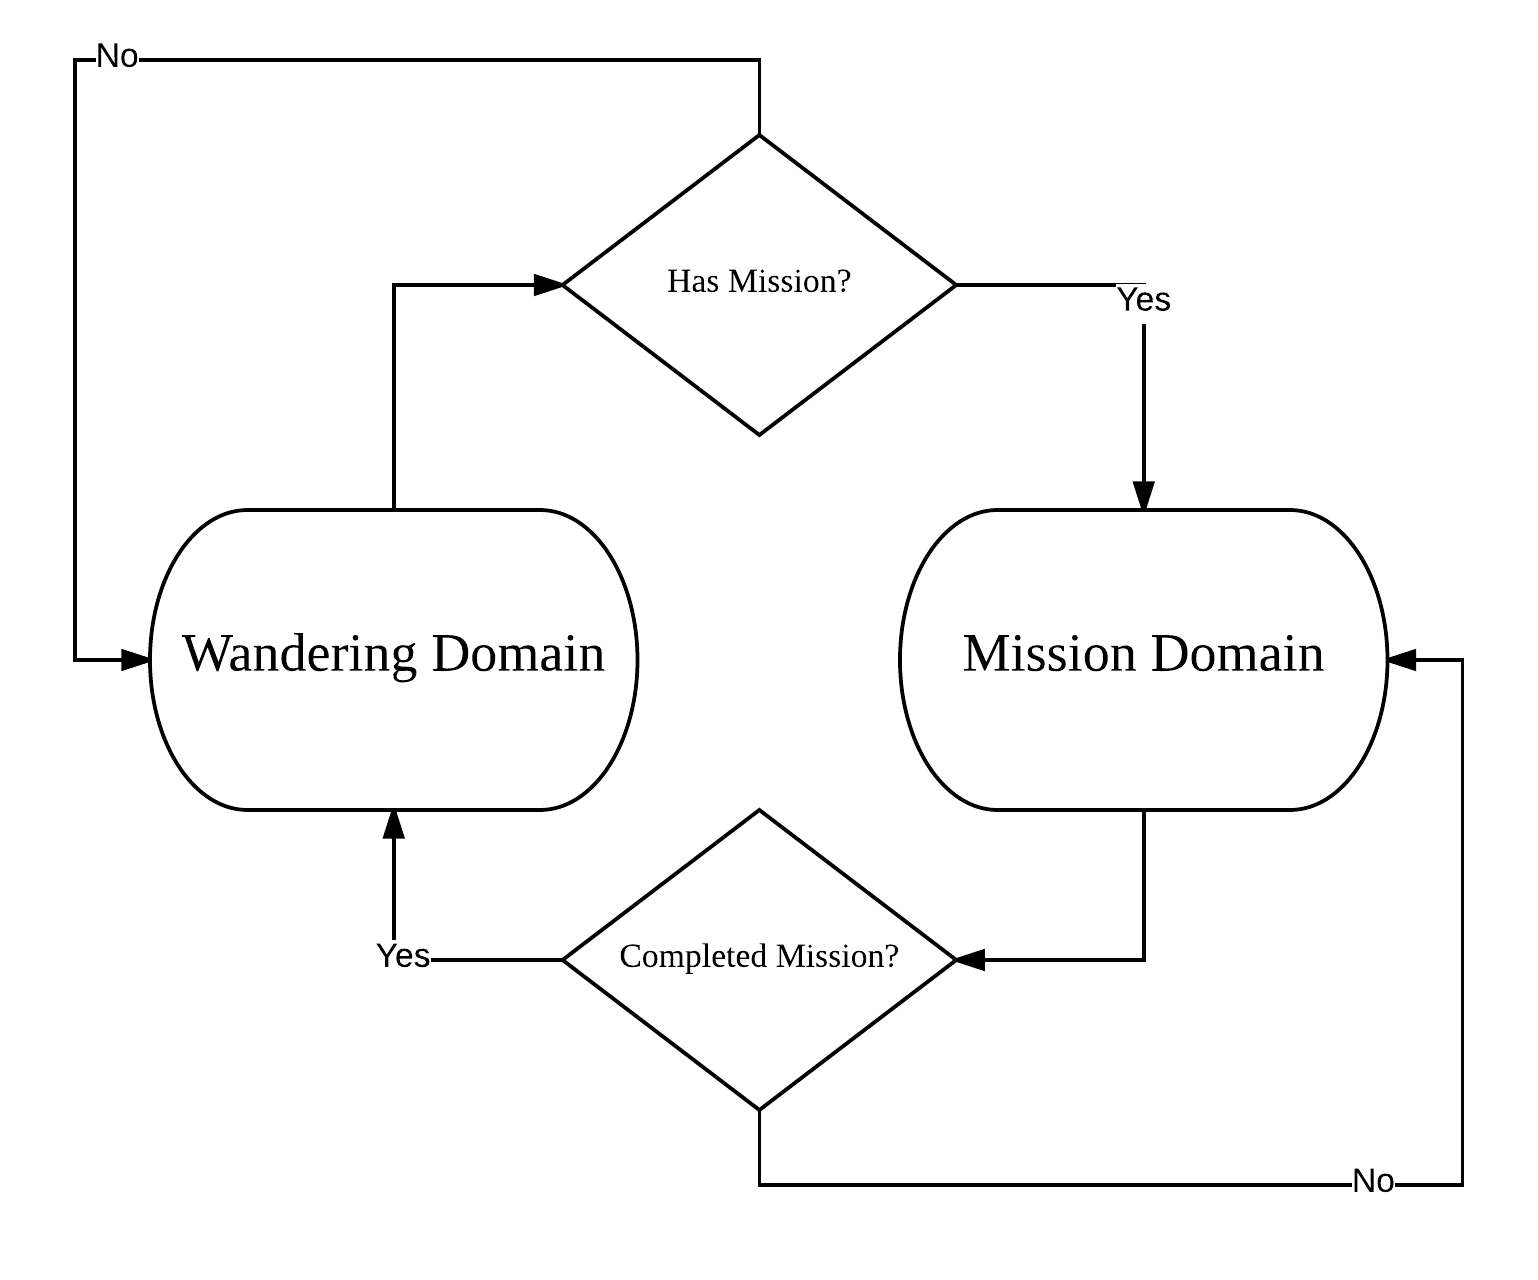
\includegraphics[scale=0.2]{images/domain_arch}
        \caption{Schematic of the domain architecture.}
        \label{fig:domain_arch}
\end{figure}

\subsubsection{Time Invariant Predicates}

The following table describes every predicate which remains static along the running 
time of the described domain. They exist for sole purpose of supporting other 
dynamic state predicates.

\begin{table}[H]
    \begin{tabularx}{\textwidth}{ |c|c|X| }
     \hline
     Predicate & Arguments & Description\\
     \hline
     person   &   \textit{Name}  &  Represents a person with \textit{Name} as
     identifier.\\
     region &   \textit{Name}   & Describes a region in the map with
     \textit{Name} as identifier.\\
     object &   \textit{Name}   & Identifies an object on the world with
     \textit{Name} identifier.\\
     robot  &   \textit{Name}   &   Tags the robot called \textit{Name}.\\
     agent &    \textit{Name}   &   An agent identified as \textit{Name} could
     be a robot, person or object.\\
     movable\_agent &   \textit{Name}   &   A movable agent identifiable by
     \textit{Name} is an agent which has movement capabilities. This means that
     an object is not a movable agent.\\
     other\_agent   &   \textit{Name}   &   It is an agent called by
     \textit{Name} apart from the robot. In other words, objects and people are
     other agents.\\
     want   &   \textit{Name,Type}  &   The agent called \textit{Name} wishes
     \textit{Object}.\\
     goal   &   \textit{Desire} & It identifies \textit{Desire} as a goal.\\
     \hline
    \end{tabularx}
    \caption{Description of predicates that are static with respect to time
    changes and that are the same in both subdomains of the model.}
    \label{table:static_predicates}
\end{table}

\subsection{Wandering Domain Description}

On this domain, the robot is wandering around the domestic environment while 
awaiting for requests given by other human agents. The robot can hear people 
calling for him (i.e. \textit{"Robot come here!"}). Additionally, he is always aware 
of the location of each agent in the scene (including himself), and their position is static (apart from
the robot). Additionally, when the 
robot moves to another room which has a person in it, there is a chance that he will be near 
that same person. 
Furthermore, the robot can engage in conversation with a person if the latter has called him earlier 
and is near him. 
While on conversation, the human may request an object, assigning a mission to him upon
the respective validation. Available predicates which comprise the full joint state are 
described in table \ref{table:dyn_preds_wandering} along with the possible actions that 
can be performed by the robot in table \ref{table:actions_wandering}. When a mission is
assigned to the robot, the current working domain switches to the Mission Domain.

\begin{table}[H]
    \begin{tabularx}{\textwidth}{ |c|c|c|X| }
     \hline
     Predicate & Arguments &  Possible Values  & Description\\
     \hline
     dynamic\_state   &  -  &   \{idle, conversation(\textit{Name})\}    &
     Indicates the operation mode of the
     robot. It can be in either two different states: \textbf{idle}, where it
     stays still for a defined period of time; or in \textbf{conversation} with
     a person identified as \textit{Name}.\\
     called &   -   &   \{none, \textit{Name}\}  &   It can indicate one of two
     things: nobody called the robot (here represented by \textbf{none}), or
     that some person with \textit{Name} called it. \\
     located    &   \textit{Name}   &   \{\textit{Region}\} & This predicate
     defines the location of agent identified as \textit{Name} in the map. It
     has the value of \textit{Region} in which the agent is located.\\
     near   &   \textit{Name}   &   \{\textit{true, false}\}    &   It indicates
     that the robot is near (or not) of person identified as \textit{Name}.  \\
     listened   &   -   &   \{\textit{(none,none), (Name, Goal) }\} &
     This predicate indicates that the robot listened (or not) to a
     \textit{Goal} command from person identified as \textit{Name}.\\
     mission    &   -  &    \{none, Desire\}  &   It represents the current
     goal of the robot. It can have two types of values: \textbf{none}, if it
     does not have any goal yet; or \textit{Desire}, if it already has a goal
     defined.\\
     \hline
    \end{tabularx}
    \caption{Time variant predicates used for the wandering domain.}
    \label{table:dyn_preds_wandering}
\end{table}



\begin{table}[H]
    \begin{tabular}{ |c|c|c|c| }
     \hline
     Action & Arguments & Description & Cost\\
     \hline
     navigate   &   \textit{Region}  &   The robot will navigate to a specified
     \textit{Region} on its map. & 8\\
     wait   &   -   &   The robot waits until new action is executed. & 5\\
     respond & \textit{Person}, \textit{ready\_to\_help} & The robot
     acknowledges a call from \textit{Person}. & 7\\
     respond & \textit{Person}, confirm\_mission, \textit{Desire} & The robot
     confirms the \textit{Desire} request from \textit{Person}. & 7\\
     \hline
    \end{tabular}
    \caption{Actions that can be performed by the robot on the wandering domain of 
    the domestic environment.}
    \label{table:actions_wandering}
\end{table}

In order to truly understand the devised model it is important to explain some of the \glspl{DDC}
which are defined in the domain.
One of them is the \textbf{navigate action}:

\begin{align*} 
    effect\_navigate(Name)_t \sim finite([0.85:NewPlace, 0.15:none]) \leftarrow \\
    robot(Name), action(navigate(NewPlace)).
\end{align*}

\begin{align*} 
    effect\_navigate(Other)_t \sim val(none) \leftarrow \\
    person(Other).
\end{align*}  

It was necessary to introduce the intermediary state predicate \textit{effect\_navigate/1} in order 
to modify the location of both person or human when holding an object, otherwise the object would
remain in the same place. Though in this case, neither people or objects can move to other places, 
as can be seen in the previous \gls{DDC} (the clause related to the object is similar to this one). 
The robot can either move to a new place with high probability or remain in the same location with 
a slight probability. The following two clauses just generate the new location of each agent according 
to the \textit{effect\_navigate/1} state predicate.

\begin{align*} 
    located(Name)_{t+1} \sim val(NewPlace) \leftarrow \\
	movable\_agent(Name), region(NewPlace),\\
    \simeq(effect\_navigate(Name)_t) = NewPlace.
\end{align*}

\begin{align*} 
    located(Name)_{t+1} \sim val(OldPlace) \leftarrow \\
	movable\_agent(Name), region(OldPlace),\\
    \simeq(effect\_navigate(Name)_t) = none,\\
    \simeq(located(Name)_t) = OldPlace.
\end{align*}

Since it is necessary to enumerate what happens to every state predicate in the model when an action is 
performed, the \textit{effect\_navigate/1} will have a \gls{DDC} for every possible action. The following 
clauses show exactly that:

\begin{align*} 
    effect\_navigate(Name)_t \sim val(none) \leftarrow \\
	robot(Name), action(wait).
\end{align*}

\begin{align*} 
    effect\_navigate(Name)_t \sim val(none) \leftarrow \\
	robot(Name), person(Other), \\
    action(respond(Other, ready\_to\_help)).
\end{align*}

\begin{align*} 
    effect\_navigate(Name)_t \sim val(none) \leftarrow \\
	robot(Name), person(Other), goal(Message), \\
    action(respond(Other, confirm\_mission, Message)).
\end{align*}

The action navigate is the only action which can modify the robot's location from one step 
to another. This is a simplification of the wandering domain and it is not true in following 
section.
This exact procedure is followed in order to describe the remaining combination of actions 
and state predicates. 
The only exception to this rule is the state predicate near:

\begin{align*} 
    near(Other)_t \sim finite([0.7:true, 0.3:false]) \leftarrow \\
	robot(Name), person(Other), \\
    \simeq(located(Name)_t) = Place, \\
    \simeq(located(Other)_t) = Place.
\end{align*}

\begin{align*} 
    near(Other)_t \sim val(false) \leftarrow \\
	robot(Name), person(Other), \\
    \simeq(located(Name)_t) = Place1, \\
    \simeq(located(Other)_t) = Place2, \\
    not(Place1 = Place2).
\end{align*}

The \textit{near/1} is only dependent on the current values of the state predicate \textit{located/1}.
Also, the robot can be near (or not) to every agent in the domain (excluding himself). So, the number of 
grounded instances can quickly grow with the number of people and objects in the domain.
Additionally, an available action is defined as applicable in that time step if it satisfies the body, of its 
action clause. For example, the action \textit{respond/2} has the following clause:

\begin{align*} 
    applicable(respond(Other, ready\_to\_help))_t \leftarrow \\
    person(Other), \\
	\simeq(near(Other):t) = true.
\end{align*}

It is only available when the robot is near to other person. It also has the following cost:

\begin{align*} 
    reward_t \sim val(-7) \leftarrow \\
	action(respond(Other, ready\_to\_help)).
\end{align*}

Finally, the goal of the domain is reached when:

\begin{align*} 
    stop_t \leftarrow \\
    goal(Purpose), \\
    \simeq(mission_t) = Purpose.
\end{align*}

And the agent receives a reward:

\begin{align*} 
    reward_t \sim val(100) \leftarrow \\
	stop_t.
\end{align*}


\subsection{Mission Domain Description}

The mission domain includes a pick-up challenge for the robot, assigned before by a human
in the domestic environment. It includes a complete action description which enables him
to pick and deliver the object himself or request help to another human while implicitly
waiting to receive it. It also describes a special rule which penalizes requests for help 
to the same human that requested the object. It is important to mention that in our 
scenario a human cannot deny a request for help and its cost is the same for all available 
people in the house (apart for the human who requested the object in the first place). This
behavior could be improved, but in this case, the description of the domain would have a higher
degree of complexity and it would take a longer time to plan which was already a limiting factor for the
current design. The predicates of the robot state and actions are also described in tables
\ref{table:dyn_preds_mission} and \ref{table:actions_mission}, respectively. 
Similarly to the last domain, the location of every agent in the scene is known, including the object, though
now every agent in the domain can move from its original location.
Finally, the mission  will persist until the human who requested the object is in possession of it, 
switching to the Wandering Domain upon completion.

\begin{table}[H]
    \begin{tabularx}{\textwidth}{ |c|c|c|X| }
     \hline
     Predicate & Arguments &  Possible Values  & Description\\
     \hline
     located    &   \textit{Name}   &   \{\textit{Region}\} & This predicate
     defines the location of agent identified as \textit{Name} in the map. It
     has the value of \textit{Region} in which the agent is located.\\
     near   &   \textit{Name}   &   \{\textit{true, false}\}    &   It indicates
     that the robot is near (or not) of person identified as \textit{Name}.  \\
     mission    &   -  &    \{none, Desire\}  &   It represents the current
     goal of the robot. It can have two types of values: \textbf{none}, if it
     does not have any goal yet; or \textit{Desire}, if it already has a goal
     defined.\\
     have & \textit{Type} & \{\textit{Name, none}\} &  A movable agent
     identified as \textit{Name} (or not) has the object with \textit{Type}. \\
     asked  &   -   &   \{\textit{(none, none), (Type, Name)}\} & The robot
     asked for help to person identified as \textit{Name} to pick object
     \textit{Type}.\\
     \hline
    \end{tabularx}
    \caption{Time variant predicates used for the mission domain.}
    \label{table:dyn_preds_mission}
\end{table}

\begin{table}[H]
    \begin{tabular}{ |c|c|c|c| }
     \hline
     Action & Arguments & Description & Cost\\
     \hline
     navigate   &   \textit{Region}  &   The robot will navigate to a specified
     \textit{Region} on its map. & 7\\
     wait   &   -   &   The robot waits until new action is executed. & 5\\
     grasp  &    \textit{Object}     & The robot picks \textit{Object}. & 25\\
     deliver    &   \textit{Object}, \textit{Person}  & The robot delivers
     \textit{Object} to \textit{Person}. & 6\\
     ask\_help   &   \textit{Object}, \textit{Person}  & The robot requests help
     from \textit{Person} in order to get \textit{Object}. & 6\\
     receive    &   \textit{Object}, \textit{Person}  & The robot receives
     \textit{Object} from \textit{Person}. & 6\\
     \hline
    \end{tabular}
    \caption{Actions that can be executed by the robot on the mission domain of 
    the domestic environment.}
    \label{table:actions_mission}
\end{table}

This domain is rather similar to the previous one, since it previously was just one 
domain. Though it was simplified by reducing the number of state predicates available
to be grounded. Also, now every agent can move from one place to another (though objects 
cannot freely move without assistance from a human or the robot). The same clauses apply 
for the robot movement, but now a person can also move, so their clauses need to be replaced.
Though, the person's movement is conditioned by the value of one state predicate: \textit{asked/0}.
It indicates if the robot requested help to this person in order to fetch an object. The action 
\textit{ask\_help/2} triggers that change in the state predicate.

\begin{align*} 
    asked_{t+1} \sim val((Type, Other)) \leftarrow \\
    object(Type), person(Other), \\
    \simeq(near(Other)_t) = true, \\
    action(ask\_help(Type, Other)).
\end{align*}

This state transition is completely deterministic. But in reality, it should not be like that and the human 
agent could have the possibility to refuse the help request. But, this was the followed approach to reduce the 
complexity of the domain. The help request becomes fulfilled when the robot has the object it wanted:

\begin{align*} 
    asked_{t+1} \sim val((none, none)) \leftarrow \\
    object(Type), person(Other), robot(Name),\\
    \simeq(asked_t) = (Type, Other), \\
    \simeq(have(Type)_t) = Name.
\end{align*}

And if the robot still is not in possession of the object, the request will remain active:

\begin{align*} 
    asked_{t+1} \sim val((Type, Other)) \leftarrow \\
    object(Type), person(Other), \\
    \simeq(asked_t) = (Type, Other), \\
    \simeq(have(Type)_t) = none.
\end{align*}

\begin{align*} 
    asked_{t+1} \sim val((Type, Other)) \leftarrow \\
    object(Type), person(Other), person(Other2),\\
    \simeq(asked_t) = (Type, Other), \\
    \simeq(have(Type)_t) = Other2.
\end{align*}

The robot can only request for help if it is near the person he wants to ask for help and if it
is not already in possession of the wanted object.
The movement of the person who has been requested to help is directed to the object location. The 
person will get the object when it is near him and then deliver it back to the robot (the person 
will move to the robot's location if he is not in the same place as it). The person performance is 
completely deterministic.
The most important clauses related to these behavior are shown below:

\begin{align*} 
    effect\_navigate(Other)_t \sim val(Place1) \leftarrow \\
    person(Other), region(Place1), region(Place2), object(Type), \\
    \simeq(asked_t) = (Type, Other), \\
    \simeq(have(Type)_t) = none, \\
    \simeq(located(Type)_t) = Place1, \\
    \simeq(located(Other)_t) = Place2, \\
    not(Place1 = Place2).
\end{align*}

\begin{align*} 
    have(Type)_{t+1} \sim val(Other) \leftarrow \\
    object(Type), person(Other), region(Place), \\
    \simeq(have(Type)_t) = none, \\
    \simeq(asked_t) = (Type, Other), \\
    \simeq(located(Type)_t) = Place, \\
    \simeq(located(Other)_t) = Place.
\end{align*}

\begin{align*} 
    effect\_navigate(Other)_t \sim val(Place1) \leftarrow \\
    person(Other), region(Place1), region(Place2), object(Type), robot(Name), \\
    \simeq(located(Name)_t) = Place1, \\
    \simeq(located(Other)_t) = Place2, \\
    \simeq(have(Type)_t) = Other, \\
    \simeq(asked_t) = (Type, Other), \\
    not(Place1 = Place2).
\end{align*}

When the person has the object is near to the robot, the latter has the oportunity to get the object 
from him, by using the action \textit{receive/2}. The other alternative the robot has is to pick the 
object by himself, when using the action \textit{grasp/1} , given by the following clause:

\begin{align*} 
    have(Type)_{t+1} \sim finite([0.7:Name, 0.3:none]) \leftarrow \\
    object(Type), person(Other), robot(Name), \\
    \simeq(have(Type)_t) = none, \\
    \simeq(asked_t) = (none, none), \\
    \simeq(near(Type)_t) = true, \\
    action(grasp(Type)).
\end{align*}

\subsection{Software Architecture}
The developed architecture (in figure \ref{fig:software_workflow}) is composed of the following components:
\begin{itemize}
	\item \textbf{Monitor Module:} receives external sensor data from multiple 
    sources, 
    processes and combines it with internal sensor data to form the joint state 
    at each time step of the run. In order to procedurally accomplish this goal, 
    the internal state is continuously tracked and modified according to the 
    result of each action. Regular expressions were used in order to parse the
    external sensor data. The module is also responsible for generating the
    grounded MDP problem from the joint state and cleaning the previous one. 
    When a problem is generated, it calls the next Module;
    \item \textbf{HYPE Module:} just a python wrapper for calling the HYPE planner
    with the desired domain and parameters: number of samples and episode depth.
    \item \textbf{Executor Module:} it receives the action to be performed from 
    the previous module, parses it and sends a ROS action message to the respective
    action server. It was used a \textit{movebase} server which was already
    integrated on the robot in order to send the robot to previously recorded 
    waypoints on the map. 
\end{itemize}

\begin{figure}[H]
    \centering
        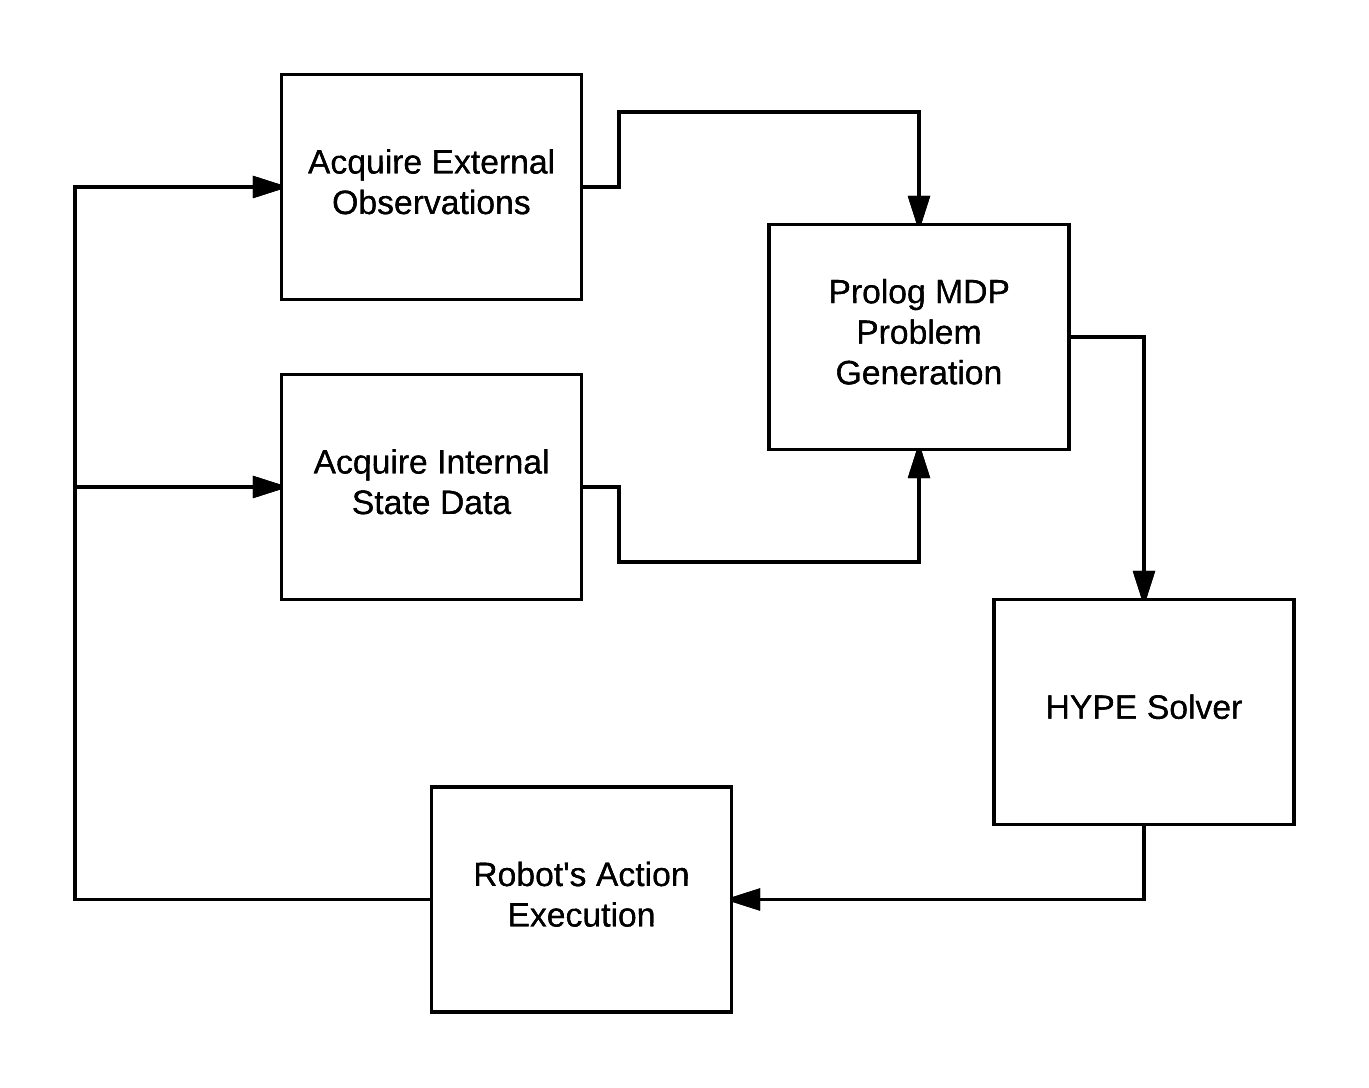
\includegraphics[scale=0.7]{images/workflow}
        \caption{High level diagram of the execution workflow.}
        \label{fig:software_workflow}
\end{figure}

In order to improve the performance of the developed module
(the planner frequently causes CPU hogging), the workload was distributed between two 
computers on a single ROS network, using a remote master on the laptop which was responsible 
for running the \textbf{HYPE Module}, as shown in figure \ref{fig:hardware_communication}. 
The rest of the ROS network ran on the robot's on-board computer. 

\begin{figure}[H]
    \centering
        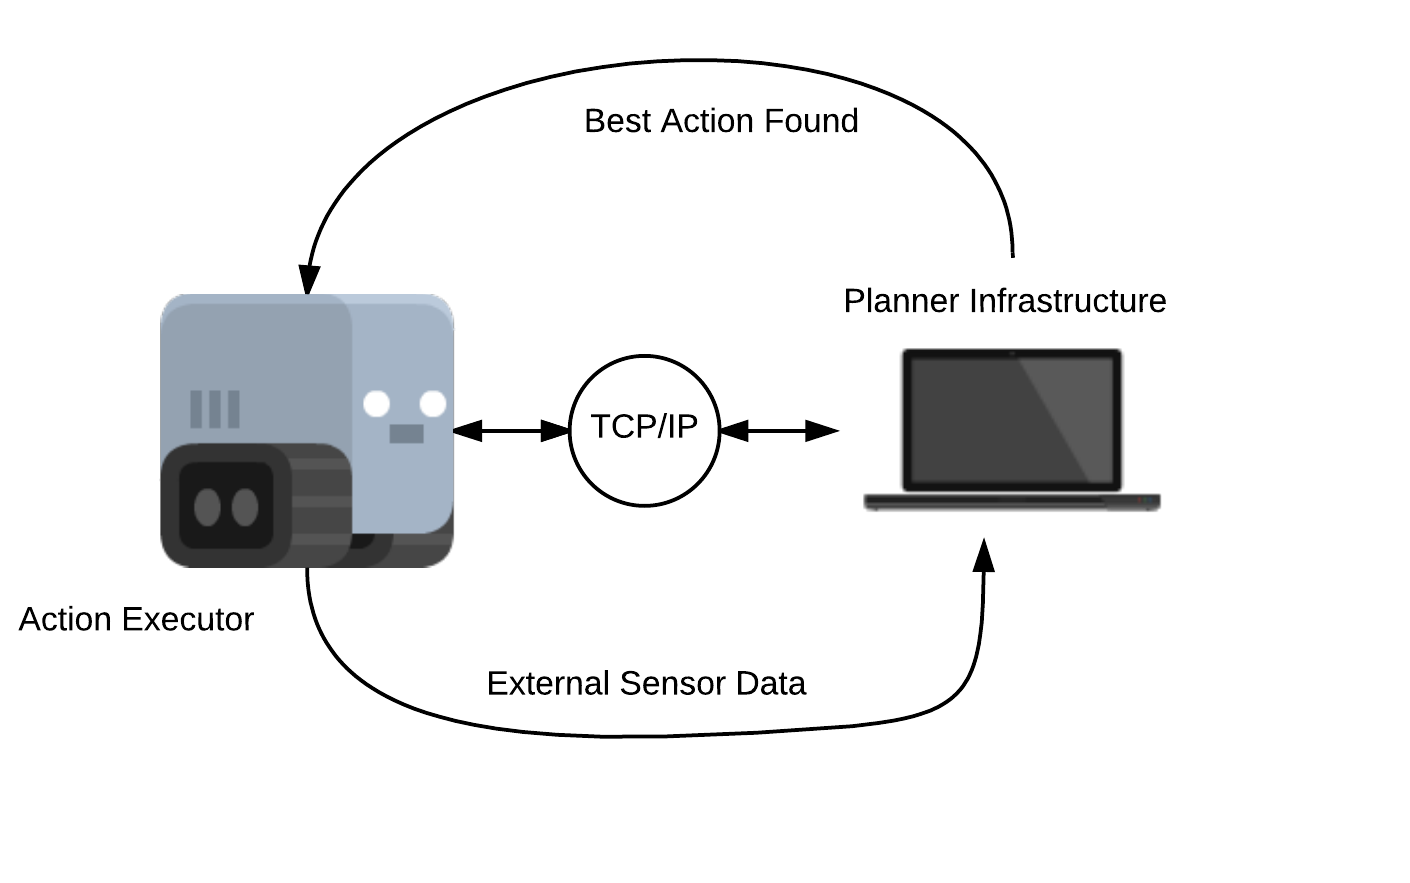
\includegraphics[scale=0.19]{images/communication}
        \caption{High level overview of the communication between hardware
        systems.}
        \label{fig:hardware_communication}
\end{figure}
